\documentclass[12pt, twoside]{article}
\usepackage[utf8]{inputenc}
\usepackage[english,russian]{babel}
\usepackage{amsmath, bm}
\newcommand{\hdir}{.}

\usepackage[unicode, pdftex]{hyperref}

\usepackage{graphicx}
\usepackage{caption}
\usepackage{amssymb}
\usepackage{amsmath}
\usepackage{mathrsfs}
\usepackage{euscript}
\usepackage{upgreek}
\usepackage{array}
\usepackage{theorem}
\usepackage{graphicx}
\usepackage{subfig}
\usepackage{caption}
\usepackage{color}
\usepackage{url}


\DeclareMathOperator*{\argmin}{arg\,min}
\DeclareMathOperator*{\argmax}{arg\,max}

\usepackage[left=2cm,right=2cm,top=3cm,bottom=2cm,bindingoffset=0cm]{geometry}

\usepackage{fancyhdr}
\pagestyle{fancy}
\fancyhead{}
\fancyhead[LE,RO]{\thepage} 
\fancyhead[CO,CE]{Анализ данных}
\fancyhead[LO,LE]{Грабовой Андрей}

\begin{document}

\begin{center}
{\LARGE \bf Методическое пособие}\\
\end{center}

\section{Обзор архитектуры исполнения и компиляции программы.}
\section{Сложность вычислений. O-нотация.}

\subsection{Методы сравнения программ}

\begin{itemize}
	\item Время работы
	\item Количеством использованной памяти
\end{itemize}

Как можно сравнивать программы решающие одну и туже задачу? Первое что хочется сказать это сколько времени программа отрабатывает на компьютере, но это не совсем так, так как вместе с вашей программой на нем работает еще очень много других программ. Для этого будем использовать не просто время работы программы, а время которое затратил процессор на нашу программу. Дальше всегда будем предполагать, что время работы программы это время затраченной процессором на выполнения только нашей программы.\\

От чего зависит время работы программы? Конечно же время работы программы зависит от мощности компьютера и тому подобное, но так-как мы договорились, что время работы это количество времени которое затратит процессор, то здесь уже явная зависимость от компьютера отпадает. На самом деле нас интересует зависимость времени работы программы от входных данных, а точнее от их размера.\\

В дальнейшем, чтобы отойти немного от компьютера введем понятия алгоритм.

\paragraph{Определение 1:} Алгоритм - это некоторая последовательность действий, которая преобразует начальные данные (input data) в выходные данные (output data).\\

Введя понятия алгоритм мы будем сравнивать не программы выполняемые на компьютере а некоторые математические модели.\\

Для простоты сравнения алгоритмов рассматривается асимптотическое сравнение двух алгоритмов. То есть как ведет себя алгоритм при изменении размера входных данных.

\paragraph{Определение 2:} Говорят, что $f(n) \in O(g(n))$, если 
$$\exists C, N:\forall n>N \rightarrow f(n) < Cg(n), \eqno(1)$$

\paragraph{Определение 3:} Говорят, что $f(n) \in \Omega(g(n))$, если 
$$\exists C, N:\forall n>N \rightarrow f(n) > Cg(n), \eqno(2)$$

\paragraph{Определение 4:} Говорят, что $f(n) \in \Theta(g(n))$, если $f(n) \in \Omega(g(n))$ и $f(n) \in O(g(n))$.\\

Введем некоторые функции, которые будут полезны для оценки сложности алгоритмов. Первой функцией является функция времени работы алгоритма от размера входа. Второй функцией является функция памяти используемой алгоритмом от размера входа.

\paragraph{Определение 5:} $T(n)$ --- это время работы алгоритма на входе (input data)  длины $n$, где под длинной $n$ подразумевается длина двоичной записи входных данных.

\paragraph{Определение 6:} $M(n)$ --- это объем дополнительной памяти требуемой алгоритмом на входе (input data)  длины $n$, где под длинной $n$ подразумевается длина двоичной записи входных данных. Под дополнительной памятью подразумевается  вся память кроме входа.

\subsection{Примеры асимптотик}

\subsection{Задача}
$sum = 0$\\
$\text{for}~0<i<n~do$\\
$....sum += 1$\\

Пусть время затраченное на прибавление единицы равно $t$. Найти асимптотическое время работы алгоритма  $T_1(n)$ для этой задачи.
$$T_1(n) = \Theta(n\cdot t)$$

\subsection{Задача}
$sum = 0$\\
$\text{for}~0<i<n~do$\\
$....\text{for}~0<j<n~do$\\
$........sum += 1$\\

Пусть время затраченное на прибавление единицы равно $t$. Найти асимптотическое время работы алгоритма  $T_2(n)$ для этой задачи.
$$T_2(n) = \Theta(n^2\cdot t)$$

\subsection{Задача}
$\text{def}~\text{f}(\text{char*} str)$\\
$....\text{if}(\text{len}(str) > 0)$\\
$........\text{return}~\text{f}(str + 1)$\\
$....\text{else}$\\
$........\text{return}~0$\\

Пусть время затраченное на прибавление единицы к индексу строки равно $t_1$, время нахождения длины строки равно $t_2$. Найти асимптотическое время работы алгоритма  $T_3(n)$ для этой задачи, где $n$ это  длина строки.
$$T_3(n) = O(n\cdot (t_1+t_2))$$

\subsection{Задача}
$min = 2^{32}$\\
$arr$ --- массив размера $n$, где все числа меньше $2^{32}$\\
$\text{for}~0<i<n~do$\\
$....\text{if}(arr[i] < min)$\\
$........min = arr[i]$\\

Пусть время затраченное на сравнение двух чисел равно $t$. Найти асимптотическое время работы алгоритма  $T_4(n)$.
$$T_4(n) = O(n\cdot t)$$


\subsection{Задача}
$arr$  --- массив размера $n$\\
$\text{for}~0<i<n~do$\\
$....\text{for}~0<j<n~do$\\
$........\text{if}(arr[j] > arr[j+1])$\\
$............\text{swap}(arr[j], arr[j+1])$\\

Пусть время затраченное на сравнение двух чисел равно $t_1$, а время затрачиваемое на перемещения двух рядом стоящих элементов массива это $t_2$. Найти асимптотическое время работы алгоритма  $T_5(n)$.

$$T_5(n) = O(n^2\cdot (t_1+t_2))$$

\section{Простейшие методы оптимизации. Градиентный спуск. Линейная модель.}

\subsection{Регрессия}
$$\mathcal{D}^l = \{x_i, y_i\}_{i=1}^l, \quad x_i \in \mathbb{R},~y_i \in \mathbb{R}. \eqno(1.1)$$

Пусть имеется некоторая обучающая выборка $\mathcal{D}^l$ размера $l$ по которой мы хотим построить некоторую модель.

\paragraph{Определение 1.1:} Линейной моделью регрессии назовем функцию $\textbf{a}(x, \textbf{w})$  из (1.2), которая зависит от некоторого неизвестного параметра $\textbf{w} \in \mathbb{R}^n$.
$$\textbf{a}(x, \textbf{w}) = \sum_{j=1}^{n} w_j f_j(x), \eqno(1.2)$$
где $f_j(x)$ --- это функция которая по заданному объекту $x$ выдает $j$-й признак этого объекта.\\

Заметим, что вектор параметров $\textbf{w}$ является неизвестным и его нужно найти по заданной выборке $\mathcal{D}^l $

\paragraph{Определение 1.2:} Введем понятия функции потерь модели $\textbf{a}$ на некотором объекте $(x,y)\in \mathcal{D}^l$ следующиим образом:
$$\mathcal{L}(\textbf{w}, (x,y)) = (\textbf{a}(x, \textbf{w}) - y)^2. \eqno(1.3)$$

\paragraph{Определение 1.3:} Введем понятия функции потерь модели регрессии $\textbf{a}$ на выборке $\mathcal{D}^l$ следующим образом:
$$\mathcal{Q}(\textbf{w}) = \sum_{j=1}^{l} \mathcal{L}(\textbf{w}, (x_j,y_j)). \eqno(1.4)$$

Теперь, мы можем сформулировать задачу машинного обучения, как поиск $\textbf{w}$, такого что $\mathcal{Q}(\textbf{w})$ является минимальным. Формальная запись этого факта, это:

$$\hat{\textbf{w}} = \argmin_{\textbf{w}\in \mathbb{R}^n}\mathcal{Q}(\textbf{w}). \eqno(1.5)$$

Тогда после нахождения такого $\hat{\textbf{w}}$, мы получаем обученную линейную модель.

\subsection{Классификация}
$$\mathcal{D}^l = \{x_i, y_i\}_{i=1}^l, \quad x_i \in \mathbb{R},~y_i \in \{-1,+1\}. \eqno(2.1)$$

Пусть имеется некоторая обучающая выборка $\mathcal{D}^l$ размера $l$ по которой мы хотим построить некоторую модель.

\paragraph{Определение 2.1:} Линейной моделью классификации назовем функцию $\textbf{a}(x, \textbf{w})$  из (2.2), которая зависит от некоторого неизвестного параметра $\textbf{w} \in \mathbb{R}^n$.
$$\textbf{a}(x, \textbf{w}) = \text{sign}\sum_{j=1}^{n} w_j f_j(x), \eqno(2.2)$$
где $f_j(x)$ --- это функция которая по заданному объекту $x$ выдает $j$-й признак этого объекта.\\

\paragraph{Определение 2.2:} Введем понятия функции потерь модели классификации $\textbf{a}$ на некотором объекте $(x,y)\in \mathcal{D}^l$ следующиим образом:
$$\mathcal{L}(\textbf{w}, (x,y)) = -\textbf{a}(x, \textbf{w})\cdot y. \eqno(2.3)$$

\paragraph{Определение 2.3:} Введем понятия функции потерь модели регрессии $\textbf{a}$ на выборке $\mathcal{D}^l$ следующим образом:
$$\mathcal{Q}(\textbf{w}) = \sum_{j=1}^{l} \mathcal{L}(\textbf{w}, (x_j,y_j)). \eqno(2.4)$$

Теперь аналогично задачи регрессии сформулируем оптимизационную задачу:

$$\hat{\textbf{w}} = \argmin_{\textbf{w}\in \mathbb{R}^n}\mathcal{Q}(\textbf{w}). \eqno(2.5)$$

\subsection{Решение оптимизационной задачи}

\subsection{Производная}
$$f'(x) = \lim_{\Delta x \rightarrow 0}\frac{\Delta f}{\Delta x}. \eqno(3.1.1)$$

\begin{figure}[h!t]\center
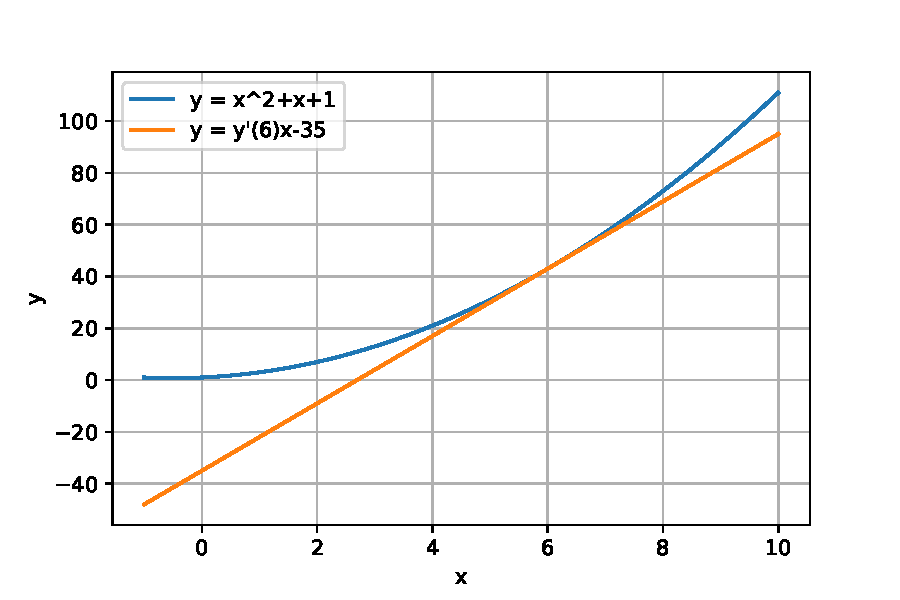
\includegraphics[width=0.7\textwidth]{section/section3_1.pdf}
\caption{График функции и касательная в точке$\textbf{a}$}
\label{Lecture_3_derivation}
\end{figure}

Будем использовать свойство знака производной. Знак производной указывает на то растет функция в этой точке или убывает, это свойство прямо следует из определения производной. Покажем этот факт:

 $$f'(x_0) =\lim_{\Delta x \rightarrow 0,~\Delta x>0}\frac{f(x_0+\Delta x) - f(x_0)}{\Delta x}, \eqno(3.1.2)$$
 
 Из уравнения (3.2) видно, что знак производной в точке $x_0$ равен знаку $f(x_0+\Delta x) - f(x_0)$, что  и требовалось показать.\\

Для примера из рис.~\ref{Lecture_3_derivation} $y'(6) = 13$. Тогда с этого следует, что функция в этой точке растет при увеличения $x$, тогда для того, чтобы найти минимальное значение $y$, нужно уменьшить $x$.\\

Вот мы пришли к выводу, что если у нас есть некоторая функция одного переменного, то для того, чтобы найти ее минимум нужно менять $x$ в противоположном направлении к знаку производной.

На этом базируется следующий итеративный подход к нахождению минимума функции.

\paragraph{Определение 3.1.1:} Итеративный процесс обозначает, что мы делаем что-то шаг за шагом.\\

Рассмотрим следующий итеративный процесс, для нахождения минимума одномерной функции $f(x)$ с областью определения $D_f$. 

1. Пусть имеется $x_0 \in D_f$ ---  некоторая точка из области определения функции.
2. Пересчитывать новую точку будем по формуле:
$$x_{n+1} = x_{n} - \alpha\cdot f'(x_{n}), \eqno(3.1.3)$$
где  $\alpha$ некоторое значение --- шаг который мы делаем, он может быть как и постоянным так и переменным. Мы будем пока считать его постоянным числом, например $0.0001$.

Мы научились находить минимум функции от скаляра. Но что же делать, для функции от вектора, которой является $\mathcal{Q}(\textbf{w})$.

\subsection{Градиент}
\paragraph{Определение 3.2.1:} Частной производной функции многих переменных $f(\textbf{x})$ по $x_j$ назовем производную функции $f'(x_j)$ считая все остальными переменные константой. Частная производная обозначается следующим образом:
$$\frac{\partial f}{\partial x_j} = f'_j(x_j), \eqno(3.2.1)$$
где $f'_j(x)$ --- это функция одной переменной, где все переменные кроме $j$-й фиксированы.

\paragraph{Определение 3.2.2:} Градиентом функции $f(\textbf{x})$ называется вектор $\nabla f(\textbf{x})$  элементы которого, это частные производные функции $f(\textbf{x})$.
$$\nabla f(\textbf{x}) = \begin{bmatrix}
\frac{\partial f}{x_1}\\
\frac{\partial f}{x_2}\\
\cdots\\
\frac{\partial f}{x_n}\\
\end{bmatrix}, \eqno(3.2.2)$$
где $x_1,~x_2,\cdots,~x_n$ --- компоненты вектора $\textbf{x}$.\\

По аналогии с функцией одного переменного можно определить итеративный процесс нахождения минимума функции многих переменных.

1. Пусть имеется $\textbf{x}^0 \in D_f$ ---  некоторая точка из области определения функции $f(\textbf{x})$.
2. Пересчитывать новую точку будем по формуле:
$$x^{n+1} = x^{n} - \alpha\cdot \nabla f(\textbf{x}^{n}), \eqno(3.2.3)$$
где  $\alpha$ некоторое значение --- шаг который мы делаем, он может быть как и постоянным так и переменным. Мы будем пока считать его постоянным числом, например $0.0001$.\\

Как видно все изменения в итеративной формуле это производная на градиент.

\subsection{Пример вычисления градиентов:}

$$f(x_1,x_2) = x_1^2 + x_2^2 \Rightarrow 
\nabla f(x_1, x_2) = \begin{bmatrix}
\frac{\partial f}{x_1}\\
\frac{\partial f}{x_2}\\
\end{bmatrix} = \begin{bmatrix}
2x_1\\
2x_2\\
\end{bmatrix}. \eqno(3.3.1)$$

$$f(x_1,x_2) = e^{x_1} + e^{x_2} + x_1x_2 \Rightarrow 
\nabla f(x_1, x_2) = \begin{bmatrix}
\frac{\partial f}{x_1}\\
\frac{\partial f}{x_2}\\
\end{bmatrix} = \begin{bmatrix}
e^{x_1}+x_2\\
e^{x_2}+x_1\\
\end{bmatrix}. \eqno(3.3.2)$$

\section{Рекурсивные алгоритмы.}
\section{Динамическое програмирование.}
\section{Простейший пример поиска в ширину на таблице.}
\section{Понятие графа. Представление графа в компьютере.}
\section{Повторение основных моделей. Автоматическое дифференцирование.}
\section{Написание модели нейронной сети при помощи python.}
\section{Работа с классами. Реализации матриц в python.}
\section{Понятие дерева. Представление дерева в памяти компютера.}
\section{Работа с изображениямии. Свертки. Реализация свертки Собеля.}
\section{Работа с деревьями. Бинарное дерево поиска.}
\section{Использование torch для обработки изображений.}
\section{Использование torch для обработки текстов. seq2seq модель.}

\href{https://github.com/andriygav/School/blob/master/2018/AD/Lecture/Lecture18.ipynb}{Ссылка на ноутбук}
\section{Использование torch для описание изображений. Image to caption task.}

\href{https://github.com/andriygav/School/blob/master/2018/AD/Lecture/Lecture17.ipynb}{Ссылка на ноутбук}


\begin{thebibliography}{99}
	\bibitem{Wine}
	\textit{Wine dataset.} http://archive.ics.uci.edu/ml/datasets/Wine
	\bibitem{Iris}
	\textit{Iris dataset.} http://archive.ics.uci.edu/ml/datasets/Iris
	\bibitem{SelfNoise}
	\textit{Self-Noise.} http://archive.ics.uci.edu/ml/datasets/Airfoil+Self-Noise
	\bibitem{Yacht}
	\textit{Yacht Hydrodynamics.} http://archive.ics.uci.edu/ml/datasets/Yacht+Hydrodynamics
\end{thebibliography}


\end{document} 